%% implementation_1_report.tex
%% V1.0
%% 2017/4/11
%% by SR Kanna, Ramcharan Sudarsanam, Preston Wipf
%%*************************************************************************

\documentclass[journal]{IEEEtran}

\usepackage[letterpaper,left=0.75in,right=0.75in,%
  top=1.5in,bottom=0.75in]{geometry}
\usepackage{listings}
\usepackage{color}
\usepackage{hyperref}
\usepackage[english]{babel}
\usepackage{graphicx}
\usepackage{caption}

\definecolor{codegreen}{rgb}{0,0.6,0}
\definecolor{codegray}{rgb}{0.5,0.5,0.5}
\definecolor{codepurple}{rgb}{0.58,0,0.82}
\definecolor{backcolor}{rgb}{0.95,0.95,0.92}

\lstdefinestyle{single}{
  backgroundcolor=\color{backcolor},
  breaklines=false,
  numbers=none,
  keepspaces=false
}

\lstdefinestyle{mystyle}{
  backgroundcolor=\color{backcolor},
  commentstyle=\color{codegreen},
  keywordstyle=\color{magenta},
  numberstyle=\color{codegray},
  stringstyle=\color{codepurple},
  basicstyle=\footnotesize,
  breakatwhitespace=false,
  breaklines=true,
  captionpos=b,
  keepspaces=true,
  numbers=left,
  numbersep=5pt,
  showspaces=true,
  tabsize=2
}

\hyphenation{op-tical net-works semi-conduc-tor}
\lstset{style=mystyle}

\begin{document}
\onecolumn

\title{Implementation 1}
\author{SR~Kanna,~Ramcharan~Sudarsanam,~Preston~Wipf}%

\markboth{Machine Learning and Data Mining, No.~1, April~2017}%
{Shell \MakeLowercase{\textit{et al.}}: Implementation 1}

\maketitle
\bigskip



\section{Problem 1}
\medskip

\section{Problem 2}
\medskip

\section{Problem 3}
\medskip

\section{Problem 4}
\medskip

\section{Problem 5}
\medskip

\section{Problem 6}
\medskip

\section{Problem 7}
\begin{figure}[!h]
\centering
\captionsetup{justification=centering,margin=2cm}
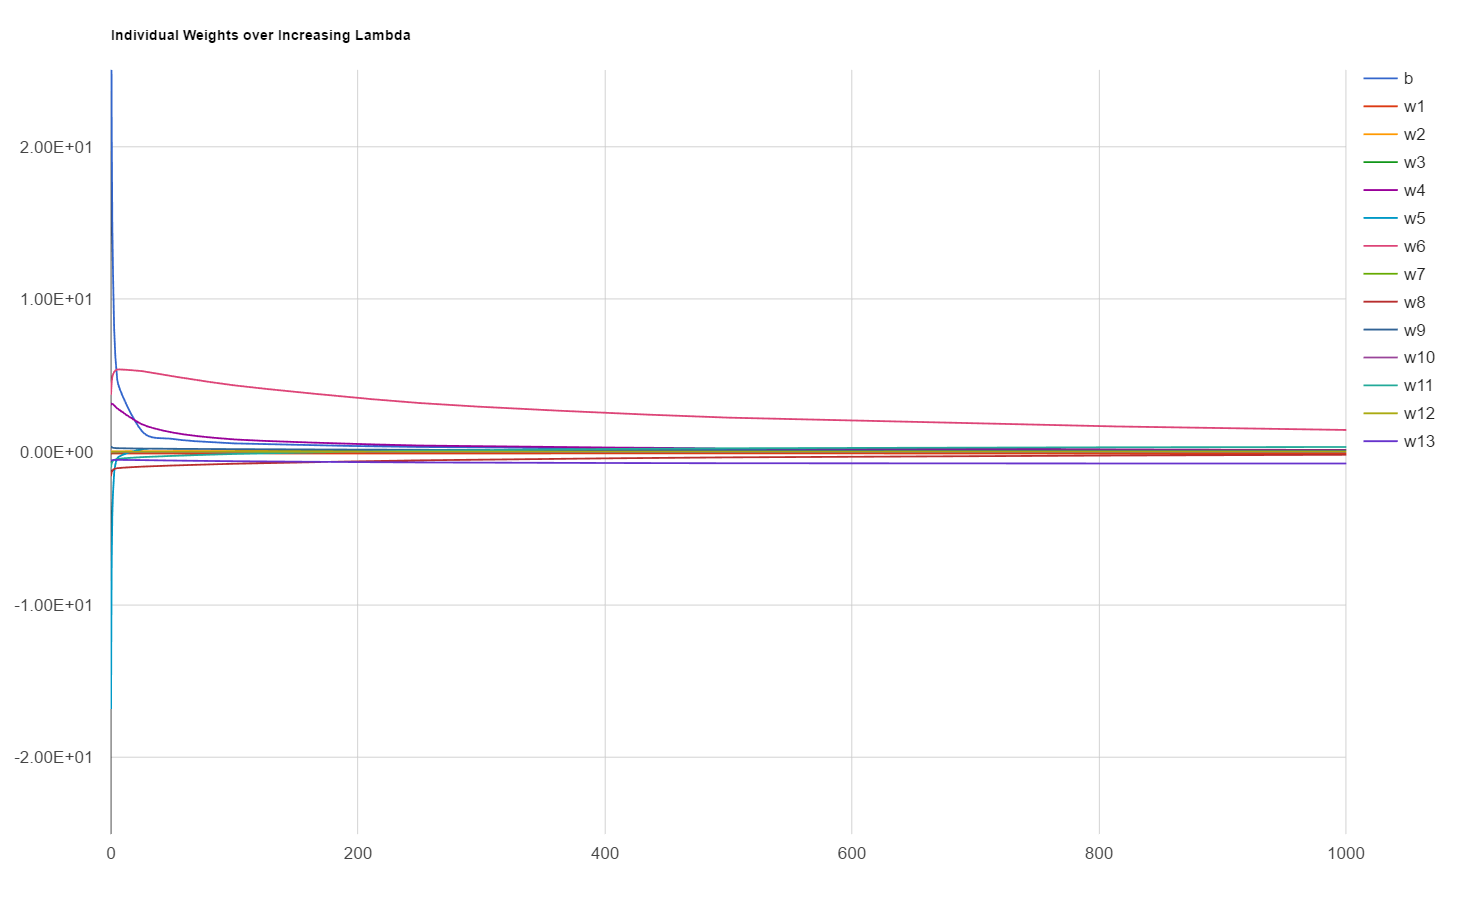
\includegraphics[width=0.95\textwidth]{weights_lambda.PNG}
\caption{\label{fig:lambdas}As you can see, the weights converge to 0 as the lambda increases.}
\end{figure}
\medskip

\section{Problem 8}
\medskip

\section{Problem 9}
\medskip

\section{Problem 10}
\medskip

 


\end{document}

